\section{Overview}
\label{sec:overview}
In this section, we motivate and demonstrate our key ideas on a simple example.

%\TODO{Reviewer: Q: Make the specification of the toy consensus (agreement) apparent.
%A: Regarding the toy example in section 2: The “essential specification” is stated in line 5 of figure 4 (the invariant labeled “safe”). Indeed, we will make this more apparent. Figure 3 is just a part of the correctness proof. We note that our approach also allows to create a more explicit "specification module" that serves as an abstract specification}

%\paragraph{Motivation}
\subsection{Example: Toy Leader Election}
\Cref{fig:toy-c} shows pseudocode for a node that participates in a
toy leader election protocol, in which a finite set of nodes decide on
a leader.  The set of nodes is a parameter of the system, which is
determined at run time and remains fixed throughout each run of the
protocol.  Each node may propose itself as a candidate by sending a
message to all nodes. Nodes vote, by sending a response message, for
the first candidate from which they receive a message. A leader is
elected when it receives a majority of the votes. This protocol will
get stuck in many cases without electing a leader. However, it
suffices to demonstrate our verification methodology, since it is
\emph{safe}, i.e., at most one leader is elected. Furthermore, a
variant of this protocol is an essential ingredient of both Raft and
Multi-Paxos, which is used in many production systems, as well as in
our evaluation.

The goal of the verification is to show that at most one leader is
elected.
%
Despite the simplicity of the property and the code, existing
verification techniques cannot automatically prove that the code is correct when executed by an unbounded
number of nodes communicating via asynchronous channels. Even when the code is annotated with invariants, the
corresponding verification conditions are expressed in undecidable
logics.
As a result, checking them with existing theorem provers such as Z3~\cite{Z3} often
results in divergence, and behaves unpredictably in general. Indeed,
previous verification efforts in the systems community identified this
as a major hurdle for verification~\cite{IronFleet}. The complexity arises due to the
combination of arithmetic, set cardinalities (e.g., number of nodes that voted for a candidate), and quantifiers in the invariant that quantify over unbounded domains
(e.g., expressing the fact that for every two nodes at most one is a
leader), especially \emph{non-stratified} quantifier alternations (see \Cref{subsec:prelims:decidable-fragments}), which give rise to potentially infinitely many instantiations.
%especially quantifier alternations, and .

\commentout{
\paragraph{Example: Toy Leader Election}
\TODO{merge}

We now explain a very simple leader election protocol, used to
demonstrate our key ideas. The protocol lets a finite set of nodes
decide on a leader. The set of nodes is a parameter of the system,
i.e., it is determined only at runtime (and remains fixed during the run of the protocol).
In the protocol, each node may propose itself as a candidate by
sending a message to all other nodes. Nodes vote, by sending a
message, to the first candidate from which they receive a message. A
leader is elected if it received a majority of the votes. This
protocol will get stuck in many cases without electing a
leader. However, it suffices to demonstrate our verification, since it
is safe, i.e., at most one leader is elected. Furthermore, a variant
of this protocol is an essential ingredient of Raft, which is used in
many production systems, as well as in our evaluation.
}

%\begin{figure}
%\begin{lstlisting}[
%    frame=single,
%    basicstyle=\scriptsize,%\footnotesize,
%    keepspaces=true,
%    numbers=left,
%    %numbersep=1em,
%    xleftmargin=2em,
%    numberstyle=\tiny,
%    emph={
%      %% assert, assume,
%      %% if, then else,
%      %% while, do,
%      %% sort, relation, function,
%      %% axiom,
%      %% insert,
%    },
%    emphstyle={\bfseries},
%    mathescape=true,
%  ]
%$\ralreadyvoted$ := false
%$\rvoters$ := $\emptyset$
%while true do {
%  msg := recv()
%  if $\text{msg.type} = \msgrequestvote \land \neg \ralreadyvoted$ {
%    $\ralreadyvoted$ := true;
%    send $\msgvote(\text{self},\text{msg.src})$
%  } else if $\text{msg.type} = \msgvote$ {
%    $\rvoters$ := $\rvoters \cup \{\text{ msg.src}\}$
%    if $\card{\rvoters} > N/2$ { send $\msgleader(\text{self})$ }
%  }
%  if $\neg \ralreadyvoted \land \text{nondet}()$ {
%    send $\msgrequestvote(\text{self})$;
%    $\ralreadyvoted$ := true
%    $\rvoters$ := $\{ \text{self} \}$
%  }
%}
%\end{lstlisting}
%\caption{\label{fig:toy-c}Toy leader election pseudocode.}
%\end{figure}

\lstset{ %
    %frame=single,
    basicstyle=\scriptsize,%\footnotesize,
    keepspaces=true,
    numbers=left,
    %numbersep=1em,
    xleftmargin=2em,
    numberstyle=\tiny,
    emph={
      %% assert, assume,
      %% if, then else,
      %% while, do,
      %% sort, relation, function,
      %% axiom,
      %% insert,
    },
    emphstyle={\bfseries},
    mathescape=true,
    frame=none
}
\lstset{emph={%
    upon%
    }
  }%

\begin{figure}
\begin{minipage}{\columnwidth}
\lstset{firstnumber=last}
\begin{tabular}{cc}
\begin{lstlisting}
// $\emph{spec: at most one node}\label{line:toy-c-spec}$
//         $\emph{sends \msgleader}$

$\ralreadyvoted$ := false
$\rvoters$ := $\emptyset$
upon client_request() do {
  if $\neg \ralreadyvoted$ {
    send $\msgrequestvote(\text{self})$
  }
}
\end{lstlisting} \hspace{0.2cm}
&
\begin{lstlisting}
upon recv(msg) do {
  if $\text{msg.type} = \msgrequestvote$
               $\land \neg \ralreadyvoted$ {
    $\ralreadyvoted$ := true;
    send $\msgvote(\text{self},\text{msg.src})$
  } else if $\text{msg.type} = \msgvote$ {
    $\rvoters$ := $\rvoters \cup \{\text{ msg.src}\}$
    if $\card{\rvoters}>N/2$ {send $\msgleader(\text{self})$}
  }
}
\end{lstlisting}
\end{tabular}
\end{minipage}
%\begin{minipage}{0.5\columnwidth}
%\hspace{0.2cm}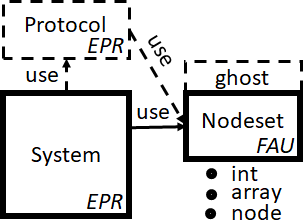
\includegraphics[scale=0.4]{fig-toy-modules-3}
%\end{minipage}
\caption{\label{fig:toy-c}Toy Leader Election pseudocode.}
\end{figure}


\subsection{Approach}
In this paper we present a verification methodology based on decidable
reasoning. We use it to develop and verify implementations of
distributed systems, whose performance is similar to other verified
implementations (e.g.~\cite{VerdiCPP}).
%, while reducing the human effort by an order of magnitude.
%obtained with tremendous human effort
%to efficient unverified implementations
%(e.g. \texttt{etcd}~\cite{etcd})
Rather than starting with an existing implementation (e.g., in C), we
define a simple imperative language which permits effective
(decidable) reasoning on one hand, and straightforward compilation
to efficient C++ code on the other hand.

%\paragraph{Modular proofs}
Our method leverages modularity in the assume-guarantee style for decidable reasoning,
%predictable automation,
by structuring the correctness proof such that different parts of the proof reason about
different aspects of the system, and at different abstraction levels, enabling each of them to
be carried out in (possibly different) decidable logics.
%Technically, this is achieved using the concept of \emph{modules} in an assume-guarantee style.
%Each module consists of procedures, pre/post-conditions and invariants, and is verified separately, while assuming the post-conditions and invariants guaranteed by other modules, in an assume-guarantee style.
The decomposition has two benefits. First, %the decomposition of the proof
it allows to reduce quantifier alternations, and eliminate bad quantification cycles. Second, it allows to check the verification conditions of each module using a different background theory (or none). % abstraction.
%n appropriate theory abstraction, making each check decidable.

\commentout{

\paragraph{Reasoning with decidable logics}
We use decidable logics to specify and check the correctness proof. This has the advantage of providing \emph{predictable} automation. In particular, when the proof is incorrect, we are able to present the user with counterexamples that make the failure visible to the user, assisting the user in fixing the proof.
However, decidable logics are rather limited. We use modularity to overcome their limitations.

\paragraph{Modular proofs}
Our method leverages modularity for decidable reasoning,
%predictable automation,
by structuring the correctness proof such that different parts of the proof are carried out in different
decidable logics. In this way, we break the undecidable problem of checking the verification conditions of the overall system
into several decidable sub-problems, each of which reasons about
different aspects of the system, and at different abstraction levels.
%
%
%Our method breaks the undecidable problem of verification
%into several decidable sub-problems, each of which reasons about
%different aspects of the system, and at different abstraction levels.
%%
%\TODO{merge with previous paragraph (repetition)} In this work we
%leverage modularity for predictable automation, by structuring the
%proof such that different parts of the proof are carried out in different
%decidable logics.
%
This is achieved using the concept of \emph{modules}.
Each module consists of procedures, pre/post-conditions and invariants, and forms a proof unit.
%Modules may be verified separately, while assuming the post-conditions and invariants guaranteed by other modules, in an assume-guarantee style. Their composition can be verified based on several proof rules.

This has two benefits. First, the decomposition of the proof allows to reduce quantifier alternations, and eliminate bad quantification cycles. Second, it allows to check the verification conditions of each module using a different theory abstraction.
%n appropriate theory abstraction, making each check decidable.
This is done by treating some symbols as interpreted inside the module that defines them, but (optionally) treating them as uninterpreted in other modules.
In this way, we decompose the proof into verification conditions that are checked independently, in different theories, and with different (stratified) quantifier alternations.
As a result, the modular proof may be checked in decidable fragments, even though the global proof would contain multiple theories and non-stratified quantifier alternations.

}
\commentout{
This is achieved by two key ideas: modularity and separate theories.

First, we decompose the verification problem into multiple subproblems, each concerning a different aspect of the proof, using the concept of \emph{modules}.
Each module consists of procedures, pre/post-conditions and invariants. The module can be understood as a lemma, which states that as long as the module's procedures are called in accordance with its preconditions, they will satisfy their postconditions, and the module invariant will be maintained.
This lemma can be used by other modules, by relying on postconditions and invariants, without inlining the proof.
Furthermore, each module (lemma) is proven separately, by checking its verification conditions.
This follows the assume-guarantee paradigm.
%This modular structure gives rise to multiple verification conditions.

The second key enabler of decidability is separation of theories. Namely, we allow to check each verification condition using an appropriate theory abstraction, making each check decidable.
This is done by treating some symbols as interpreted inside the module that defines them, but (optionally) treating them as uninterpreted in other modules.
%Furthermore, each VC can have different quantifier alternation structure, allowing each VC to be stratified, even though the global proof is not stratified.

By combining these two ideas, we decompose the proof into verification conditions that are checked independently, in different theories, and with different (stratified) quantifier alternations.
As a result, the modular proof may be checked in decidable fragments, even though the global proof would contain multiple theories and non-stratified quantifier alternations.
}

\commentout{
%\paragraph{Obtaining modular proofs of distributed systems}
\paragraph{Patterns for obtaining modular proofs}
We identify two patterns that capture common programming languages practices, and allow for a natural decidable decomposition:
%of the proof into a modular proof:
1)~Data structures
with first-order interfaces, and 2)~Protocol designs as lemmas for
proving the implementation.
We used these patterns to construct modular proofs for our examples. % enabled decidable reasoning in our examples.

\para{Data structures with first-order interfaces}
Efficient implementations deploy concrete primitive types (e.g.,
integers), which call for using theories (e.g., arithmetic) to reason about them.
Also, when it comes to distributed systems, the code of a process may be run by any number of nodes.
It is therefore natural to reason about such systems
%model unbounded (distributed) systems
in first-order logic, using quantifiers over unbounded domains (e.g., the set of nodes) and uninterpreted functions.
However, the combination of quantifiers, uninterpreted functions and,
e.g., arithmetic, often leads to undecidability. Encapsulating
primitive types in a pure (uninterpreted) first-order logic interface
decomposes the verification problem into the problem of reasoning in
uninterpreted first-order logic, where the primitive types are opaque
and only their interface is used, and reasoning about the low-level
implementation, showing that it satisfies its interface, which can be
done in decidable %(quantifier-free)
interpreted theories.

\para{Protocol designs as lemmas for proving the implementation}
Data structures with first-order interfaces simplify reasoning, but in
general, do not suffice for verifying interesting distributed systems
in decidable logics. The reason for this is that even the first-order
reasoning problem is undecidable, since proofs of complex systems
require quantifier alternation, which leads to
undecidability. Fortunately, distributed systems are constructed in an
evolutionary process starting with a protocol design, and then
gradually developing an efficient implementation, guided by the
protocol design. In this paper, we exploit this idea in a novel way,
by capturing the design and its correctness in a ghost object, which
is verified separately and serves as a lemma for proving the implementation. This provides a
natural way to further decompose the verification problem into
sub-problems, where each sub-problem usually contains fewer quantifier
alternations. In our limited experience, this usually results in each
problem becoming decidable, i.e., contain only stratified (acyclic)
quantifier alternations.

}

\commentout{
Data structures with first-order interfaces are a way to separate
reasoning about theories (e.g., arithmetic) from reasoning with
quantified first-order logic. We do this by encapsulating data
structures in a pure (uninterpreted) first order logic
specification. Each data structure is decomposed into an interface and
a corresponding implementation. The implementation is verified to
satisfy the interface using decidable (interpreted) theories capturing
features of the implementation. Properties of the implementation are
specified in pure first-order logic in order to be used in the proofs
of code using the data structure. These proofs rely solely on the
interface and result in verification conditions in quantified
uninterpreted first order logic. In this way we manage to eliminate
the need to combine quantifiers with interpreted theories. Secondly,
we decompose to reduce the reasoning over first-order quantifiers to
decidable checks, we use ghost objects to encapsulate pieces of proofs
in lemmas. Breaking a global proof into objects allows a proof
structure in which each object results in verification conditions in
first-order logic with stratified quantifier alternation, which
ensures decidability. A particularly useful way ghost objects are used
is as a way to separate the protocol design by abstracting some
implementation details, and then using the correctness of the design
as a lemma for proving the implementation correct.
}


%\subsection{Verification Friendly Modular Implementation}
\subsection{Modular Formulation}

% Modules used ...
% Modular...
%\TODO{add figure with modules}

We illustrate our methodology on the Toy Leader Election example, to verify that at most one
leader is elected using \emph{decidable} reasoning.
Our formulation of the system consists of three \emph{modules}: $\mtoyprotocol$, $\mtoysystem$, and $\mnodeset$.
The interplay between the modules and the decidable fragments in which they are verified are depicted in \Cref{fig:modules} (the fragments are defined in \Cref{sec:prelim}); their code is listed in \Cref{fig:toyprotocol,fig:toysystem,fig:nodeset}.
The code is written in {\bf M}odular {\bf D}ecidable {\bf L}anguage (\Lang) ---
an illustrative programming language enabling modular decidable verification.
% and implementation of distributed systems.

Each module should be viewed as a proof unit, which consists of
\begin{inparaenum}[(1)]
\item declarations and definitions of types and state components, which may be interpreted using \keyword{interpret} declarations,
\item declarations of other modules and their invariants that are used by the module, specified by the \keyword{uses} clause,
\item a module invariant $\modinvar$, given by all \keyword{invariant} declarations in the module,
\item procedures with pre-post specifications, specified by \keyword{requires} and \keyword{ensures} declarations (an
unspecified condition is $\true$ by default), and
\item declaration of the module's initial state, either with \keyword{init} declarations or with an $\pinit()$ procedure.
\end{inparaenum}
Intuitively, a module is correct if all its procedures satisfy their pre/post specification, and also maintain the module invariant,
assuming that the used modules are themselves correct.
The key property of the modular formulation is that verification conditions generated for each module fall into decidable fragments (see \Cref{subsec:overview:decidable}), which allows predictable automation.
%\oded{Please check last sentence}
%We note that our methodology is the first to employ decidable logics
%for reasoning all the way from protocol design to protocol
%implementation.


\commentout{
We illustrate our methodology on %a system that implements the simple leader election protocol.
the simple leader election example.
In order to facilitate \emph{decidable} reasoning for implementing and verifying the safety of this system, i.e., that at most one
leader is elected, we apply modular reasoning using the two patterns discussed above.
To that end, our formulation of the system consists of three \emph{modules}. %, where each module should be viewed as a proof unit.
The interplay between these modules and the fragments in which each of them is verified are depicted in \Cref{fig:modules}; their code is listed in \Cref{fig:toyprotocol,fig:toysystem,fig:nodeset}.
The code is written in the {\bf M}odular {\bf D}ecidable {\bf L}anguage (\Lang) ---
a language for modular decidable verification and implementation of distributed systems.
In our evaluation, we simulate {\Lang} using the Ivy language and system~\cite{Ivy,ken_fmcad16}.
}

\commentout{
\begin{figure}
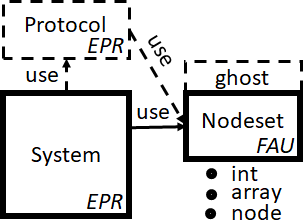
\includegraphics[scale=0.5]{fig-toy-modules-3}
\caption{Modules and built-in types used for verifying the toy example. Ghost modules (or parts of modules) are depicted using dashed lines.
Each module is annotated with the decidable fragment in which it was verified. \label{fig:modules}}
\end{figure}
}


\begin{SCfigure}
\caption{Modules and built-in types used for verifying the toy example. Dashed box denotes a ghost module.
Each module is annotated with the decidable fragment in which it is verified. \label{fig:modules}}
    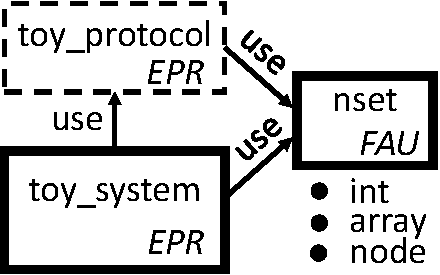
\includegraphics[scale=0.6]{modules-fig-trim}
\end{SCfigure}

We elaborate on the modules of the Toy Leader Election example in \Cref{sec:toyprotocol,sec:toysystem,sec:nodeset}.
Roughly speaking:

%In the example, t
(i) The {\mnodeset} module defines (and verifies) a data type which encapsulates sets of nodes under a first-order interface,
and hides the low-level implementation.
This allows other modules to treat sets of nodes as an opaque type, relying only on the first-order interface, so their verification can be carried out in uninterpreted first-order logic.
Verifying that the $\mnodeset$ module satisfies its interface is carried out in a suitable theory.
The first-order interface includes a predicate that tests if a set of nodes forms a majority,
along with the property that any two majorities intersect, which is crucial for the proof of the protocol.

(ii) The {\mtoyprotocol} module defines (and verifies) an abstract model of the protocol, eliding some of the
implementation details.
This is in line with the common practice of developing a system in an evolutionary process:
starting with a design, and then gradually developing an efficient implementation.
Here this practice serves a different purpose; namely, the {\mtoyprotocol} captures the protocol design and its correctness in a ghost object,
which is verified separately and serves as a lemma for proving the implementation.
This provides a natural way to decompose the verification problem,
and as we shall see, to avoid quantifier alternation cycles.

(iii) The {\mtoysystem} module specifies (and verifies) the system implementation,
using both the data type defined by $\mnodeset$ (relying on its first-order specification) and the
abstract protocol defined by $\mtoyprotocol$ (as ghost code) to obtain a verified executable implementation.

% We elaborate on these modules below.

\subsubsection{Abstract Protocol Module}
\label{sec:toyprotocol}
%\subsection{Protocol Designs as Lemmas for Proving Implementations}

\begin{figure}
\begin{lstlisting}[
    %frame=single,
    basicstyle=\scriptsize,%\footnotesize,
    keepspaces=true,
    numbers=left,
    %numbersep=1em,
    xleftmargin=2em,
    numberstyle=\tiny,
    emph={
      %% assert, assume,
      %% if, then else,
      %% while, do,
      %% sort, relation, function,
      %% axiom,
      %% insert,
    },
    emphstyle={\bfseries},
    mathescape=true,
  ]
ghost module $\mtoyprotocol$ uses $\mnodeset$, $\mnodeset.\iintersect$ { $\label{line:protocol:uses}$
  relation $\rvoted$ : $\snode,\snode$
  relation $\risleader$ : $\snode$
  variable $\rquorum$ : $\snodeset$
  init $\forall n_1,n_2. \; \neg\rvoted(n_1,n_2)$
  init $\forall n. \neg\risleader(n)$
  invariant $\ioneleader$ = $\forall n_1, n_2. \; \risleader(n_1) \land \risleader(n_2) \to n_1 = n_2 \label{line:toyprotocol-inv-1}$
  invariant $\forall n,n_1,n_2. \; \rvoted(n,n_1) \land \rvoted(n,n_2) \to n_1 = n_2 \label{line:toyprotocol-inv-2}$
  invariant $\forall n : \snode. \; \risleader(n) \to \big( \mnodeset.\rmajority(\rquorum) \, \land \label{line:toyprotocol-inv-3}$
                                     $\forall n':\snode. \; \mnodeset.\rmember(n' , \rquorum) \to \rvoted(n', n)\big)$
  procedure $\pvote(\text{v} : \snode ,\, \text{n} : \snode)$ {
    requires $\forall n'. \neg\rvoted(\text{v},n')$
    $\rvoted(\text{v}, \text{n})$ := true
  }
  procedure $\pbecomeleader(\text{n} : \snode ,\, \text{s} : \snodeset)$ {$\label{line:toyprotocol-becomeleader}$
    requires $\mnodeset.\rmajority(\text{s}) \, \land$ $\forall n':\snode. \; \mnodeset.\rmember(n' , \text{s}) \to \rvoted(n', n)\label{line:toyprotocol-becomeleader-pre}$
    $\risleader(\text{n})$ := true $\label{line:toyprotocol-becomeleader-assign-1}$
    $\rquorum$ := s $\label{line:toyprotocol-becomeleader-assign-2}$
  }
}
\end{lstlisting}
\caption{\label{fig:toyprotocol}Protocol module for Toy Leader Election.}
\end{figure}


%\TODO{add line references} \TODO{use different notation for named invariant}
\Cref{fig:toyprotocol} lists the module that formalizes the
abstract leader election protocol.
This is a ghost module, which is only used for the sake of the proof.
%, presented in {\Lang}a simplified form of the Ivy language \TODO{name the language. SH: I don't think it is necessary}.
The module contains two mutable relations that define its state:
$\rvoted(n_1,n_2)$ captures the fact that $n_1$ voted for $n_2$, and
$\risleader(n)$ means node $n$ is an elected leader. The initial state
of the module specifies that both relations are empty. The state also
includes a variable $\rquorum$, that remembers the last voting
majority observed. The abstract protocol provides a global invariant
(denoted by \keyword{invariant}), which states that there is at most
one leader. This is similar to a class invariant / object invariant in
modular reasoning. Next, the module contains a proof that all of its
reachable states satisfy the global invariant, by an inductive
invariant. When proving this module, the majority intersection
invariant of the $\mnodeset$ module is used, as indicated by the
\keyword{uses} clause in \cref{line:protocol:uses}.

The module also provides two procedures that define the abstract
protocol steps. Each procedure specifies a pre condition.
%, denoted by the \keyword{requires} and \keyword{ensures} keywords (an
%unspecified condition is $\true$ by default).
The $\pvote(n_1,n_2)$
procedure models a vote by $n_1$ for $n_2$, and its precondition is
that node $n_1$ has not yet voted. The $\pbecomeleader(n,s)$ procedure
models the election of $n$ as a leader, and its precondition requires
that all nodes in $s$ voted for $n$, and that $s$ is a majority.
%
Note that this module is abstract in the sense that it abstracts network communication and uses a global view of the system. In particular, the $\pbecomeleader$ does not specify how a node learns that it received a majority of votes.
%\TODO{Indeed, it is a \keyword{ghost} module, which is only used for the sake of the proof.}
%thus avoiding the local bookkeeping.

\commentout{
nodes have a global view of the system (e.g., via the $\rvoted$ relation), and may directly access the local state of other nodes, without exchanging messages. Clearly, such a module cannot be implemented in a distributed setting. Indeed, it is a \keyword{ghost} module, which is only used for the sake of the proof.
\TODO{emphasize in what ways it is abstract: it has global view. No messages, etc.}
}

\commentout{
%%% MOVED
During modular verification, this module will result in verification
conditions (VC's) that check: 1) $\INV$ --- the provided inductive
invariant combined with the global guarantee, holds at any initial
state, and 2) that the execution of a procedure starting from states
that satisfy $\INV$ and the precondition result in states that satisfy
$\INV$ and the postcondition. The VC's will also assume the
{\iintersect} guarantee of the nodeset datatype. Fig X lists
these verification conditions. These verification conditions contain
$\forall\exists$ quantifier alternation from nodeset to node, but this
is stratified and therefore decidable to check.

\TODO{add figure with VC's}
}

\subsubsection{Concrete Implementation Module}
\label{sec:toysystem}

\begin{figure}
\begin{lstlisting}[
    %frame=single,
    basicstyle=\scriptsize,%\footnotesize,
    keepspaces=true,
    numbers=left,
    %numbersep=1em,
    xleftmargin=2em,
    numberstyle=\tiny,
    emph={
      %% assert, assume,
      %% if, then else,
      %% while, do,
      %% sort, relation, function,
      %% axiom,
      %% insert,
    },
    emphstyle={\bfseries},
    mathescape=true,
  ]
system module $\mtoysystem$ uses $\mnodeset$, $\mtoyprotocol$, $\mtoyprotocol.\ioneleader$ { $\label{line:toysystem-uses}$
  message $\msgrequestvote$ : $\snode$  $\label{line:system:msg-def1}$
  message $\msgvote$ : $\snode, \snode$ $\label{line:system:msg-def2}$
  message $\msgleader$ : $\snode$ $\label{line:system:msg-def3}$
  // $\emph{spec: at most one node sends \msgleader}:$
  invariant $\isafe$ = $\forall n_1, n_2. \; \msgleader(n_1) \land \msgleader(n_2) \to n_1 = n_2$ $\label{line:system-guarantee}$

  relation $\ralreadyvoted$ : $\snode$ $\label{line:system-begin-node}$
  function $\rvoters$ : $\snode \to \snodeset$
  procedure $\pinit(\text{self}:\snode)$ {
    $\ralreadyvoted(\text{self})$ := false
    $\rvoters(\text{self})$ := $\mnodeset.\pemptyset()$
  }
  procedure $\prequestvote(\text{self}:\snode)$ {
    send $\msgrequestvote(\text{self})$
  }
  procedure $\pcastvote(\text{self}:\snode ,\, \text{n}:\snode)$ handles $\msgrequestvote(\text{n})$ {
    if $\neg\ralreadyvoted(\text{self})$ {
      $\ralreadyvoted(\text{self})$ := true
      send $\msgvote(\text{self}, \text{n})$
      $\mtoyprotocol.\pvote(\text{self}, \text{n})$ $\label{line:system:ghost-2}$
    }
  }
  procedure $\preceivevote(\text{self}:\snode, \text{n}:\snode)$ handles $\msgvote(\text{n},\text{self})$ {
    $\rvoters(\text{self})$ := $\mnodeset.\padd(\rvoters(\text{self}), \text{n})$
    if $\mnodeset.\rmajority(\rvoters(\text{self}))$ { $\label{line:system:majority}$
      send $\msgleader(\text{self})$
      $\mtoyprotocol.\pbecomeleader(\text{self},\rvoters(\text{self}))$ $\label{line:system:ghost-3}$
    }
  } $\label{line:system-end-node}$
  // $\emph{inductive invariant for the proof:}$
  invariant $\forall n_1,n_2. \; \mtoyprotocol.\rvoted(n_1,n_2) \leftrightarrow \msgvote(n_1,n_2)$ $\label{line:system:inv-1}$
  invariant $\forall n_1,n_2. \, \mnodeset.\rmember(n_1,\!\rvoters(n_2)) \! \to \! \mtoyprotocol.\rvoted(n_1,\!n_2)$ $\label{line:system:inv-2}$
  invariant $\forall n. \; \msgleader(n) \leftrightarrow \mtoyprotocol.\risleader(n)$ $\label{line:system:inv-3}$
  invariant $\forall n_1,n_2. \; \neg \ralreadyvoted(n_1) \to \neg \mtoyprotocol.\rvoted(n_1,n_2)$ $\label{line:system:inv-4}$
  open $\mtoyprotocol$ $\label{line:system:open}$
}
\end{lstlisting}
\caption{\label{fig:toysystem}System module for Toy Leader Election. }
\end{figure}


\Cref{fig:toysystem} lists the concrete system implementation.  We
consider systems in which a finite (but unbounded) set of nodes run
the same code, and exchange messages. For simplicity, we assume all
messages are broadcast to all nodes. Our network model also allows
message dropping, duplication and reordering. To define the system
implementation, we first define the message
types. \Cref{line:system:msg-def1,line:system:msg-def2,line:system:msg-def3}
define three message types: {\msgrequestvote} that a node uses to
propose itself as a leader, {\msgvote} that a node sends to vote for a
candidate, and {\msgleader} that a node uses to announce it is elected
as the leader. The first field of each message is its source
node.
%\ken{Following two sentences added in response to shepherd comment 3}
The invariant on \cref{line:system-guarantee} specifies the desired specification, i.e., that only
one node ever issues a {\msgleader}
message. This is the ultimate guarantee provided by the implementation,
and it is the only line of trusted specification in the
example. Namely, one has to trust that this invariant captures the intended property (e.g., by careful inspection),
but the fact that the implementation maintains it is mechanically verified.
%\sharon{I don't understand this sentence. In what sense is it trusted code? it is the invariant??}
%\oded{It's supposed to answer the reviewer's question. This line is trusted in the sense that if we wrote it wrong (suppose we had a typo that makes it equivalent to true), Ivy wouldn't catch us. Any error in any other part of the code would be caught. Maybe we can think of a better wording}
%\sharon{I think we should remove it. It is as trusted as any other invariants: all of them are verified. What is not verified is whether this logical formula captures the intent of the user, just like the code may be not exactly what the user wanted. We can just say "Unlike the other annotations, which are internal to the proof, this invariant defines the specification that is being verified (and is therefore of special interest to the user)." }
The declarations are followed by the code to be run on each node. This
code (lines \ref{line:system-begin-node} to
\ref{line:system-end-node}) defines the local state of each node, as
well as procedures that can be executed in response to client
requests, or procedures that are message handlers (specified by the
\keyword{handles} declaration), and executed upon receiving a message
from the network. The state components are defined as functions (or
relations) whose first argument is a node, so that $f(n)$ denotes the
local state of node $n$.  Similarly, all procedures receive as their
first argument the {\self} identifier of the node that runs them.
Since the system module is going to be compiled into an executable
code that runs on each node, we syntactically enforce that each node
may only access and modify its own local state.
% (via the {\self} identifier).

We note that the $\mtoysystem$ module makes use of the $\mnodeset$
module to maintain sets of voters, and uses a majority test
(\cref{line:system:majority}). It also makes calls into the ghost
module $\mtoyprotocol$
(\cref{line:system:ghost-2,line:system:ghost-3}). This allows to
establish an invariant that relates the state of the concrete module
and the abstract module
(\cref{line:system:inv-1,line:system:inv-2,line:system:inv-3,line:system:inv-4}),
and use the proven invariant of the abstract module as a lemma for
proving the concrete implementation. This is indicated by the
\keyword{uses} clause, which declares use of the
$\mtoyprotocol.\ioneleader$ invariant (\cref{line:toysystem-uses}).

%\subsubsection{Data Structures with First-Order Interfaces}
\subsubsection{Node Set Module}
\label{sec:nodeset}

\begin{figure}
\begin{lstlisting}[
    %frame=single,
    basicstyle=\scriptsize,%\footnotesize,
    keepspaces=true,
    numbers=left,
    %numbersep=1em,
    xleftmargin=2em,
    numberstyle=\tiny,
    emph={
      %% assert, assume,
      %% if, then else,
      %% while, do,
      %% sort, relation, function,
      %% axiom,
      %% insert,
    },
    emphstyle={\bfseries},
    mathescape=true,
  ]
module $\mnodeset$ {
  type t
  relation $\rmember$ : $\snode,\text{t}$
  relation $\rmajority$ : t
  function $\risize$ : t $ \to \sint$

  interpret t as array<$\sint$,$\snode$> $\label{line:nodeset-t}$
  interpret $\rmember(n,s)$ as $\exists i. 0 \leq i < \rlen(s) \land \rvalue(s,i,n)$ $\label{line:nodeset-member}$
  interpret $\rmajority(s)$ as $\risize(s) + \risize(s) > \risize(\rallnodes)$ $\label{line:nodeset-majority}$

  invariant $\iintersect$ = $\forall s_1, s_2. \; \rmajority(s_1) \land \rmajority(s_2) \,\to$ $\label{line:nodeset-intersect}$
                            $\exists n. \; \rmember(n, s_1) \land \rmember(n, s_2)$

  procedure $\pemptyset()$ returns s:t {
    ensures $\forall n. \; \neg\rmember(n,\text{s})$
    s := array.empty()
  }
  procedure $\padd(\text{s}_1 : \text{t} ,\, \text{n} : \snode)$ returns $\text{s}_2 : \text{t}$ {
    ensures $\forall n'. \; \rmember(n', \text{s}_2) \leftrightarrow (\rmember(n', \text{s}_1) \lor n' = n)$
    if $\rmember(\text{n}, \text{s}_1)$ then { $\text{s}_2$ := $\text{s}_1$ } else { $\text{s}_2$ := array.append($\text{s}_1$, n) } $\label{line:nodeset-append}$
  }
  procedure $\pinit()$ {
    $\risize$ := $\lambda x. 0$;
    for $0 \leq i < \rlen(\rallnodes)$ {
      invariant $\forall s_1,s_2. (\forall n. \neg (\rmember(n,s_1) \land \rmember(n, s_2))) \, \to$ $\label{line:nodeset-inv}$
          $\risize(s_1) + \risize(s_2) \leq \risize(\rallnodes)$
      $\risize$ := $\lambda x. \big( (\risize(x) + 1)$ if $\rmember(\text{array.get}(\rallnodes,i),x)$ else $\risize(x)\big)$ $\label{line:nodeset-lambda}$
    }
  }
}
\end{lstlisting}
\caption{\label{fig:nodeset}The $\mnodeset$ module for node sets, proving the majority intersection property.}
\end{figure}

\commentout{
  ghost relation $\rreachedset$ : t
  interpret t as array<$\sint$,$\snode$> with $\rreachedset$
  interpret $\rreachedset(s)$ as $\rlen(s) = \risize(s)$

  invariant $0 \leq i \leq \rlen(\rallnodes)$

}



\Cref{fig:nodeset} lists the code for the $\mnodeset$ module. This
module defines a data structure for storing sets of nodes, with
operations for adding to a set and testing whether a set is a
majority. To do so, it defines a type t, whose internal interpretation is \Lang's
built-in array, as declared in \cref{line:nodeset-t}.
%The implementation uses \Lang's built-in arrays as a
%naive implementation for sets.
Sets are created using the $\pemptyset$ and $\padd$ procedures, which
provide a naive implementation of a set, stored as an array of its
elements.  The module defines the $\rmember$ relation, and provides it
with an interpretation via an \keyword{interpret} declaration in
\cref{line:nodeset-member}. As we shall see, this definition creates
an executable membership test that is translated to a loop that scans
the array.

Most importantly for verifying the leader election modules, the
$\mnodeset$ module provides the interpreted $\rmajority$ predicate,
with the key property that any two majorities intersect. This is
stated by the $\iintersect$ invariant (\cref{line:nodeset-intersect}).
Intuitively, a set is a majority if its cardinality is more than half
the total number of nodes.  In \Cref{fig:nodeset}, the $\rmajority$
predicate is interpreted using the $\risize$ function to compute the
cardinality of a set of nodes, and the built-in value $\rallnodes$,
which is an array with the special semantics that it contains all
nodes.  The $\risize$ function computes the cardinality of a set of
nodes, and it is constructed in the $\pinit()$ procedure of the
$\mnodeset$ module in a way that establishes the majority intersection
property. The proof is by induction, manifested in the loop invariant
in \cref{line:nodeset-inv}.

We note that the loop in $\pinit()$ constructs $\risize$ via a nesting
of $N$ function closures (where $N$ is the number of nodes). This
definition of $\risize$ allows an easy proof of the majority
intersection property (the $\lambda$ at \cref{line:nodeset-lambda} is eliminated from verification conditions by $\beta$-reduction, resulting in first-order formulas; see \Cref{sec:extensions}). A more efficient implementation uses $\rlen$
(underlying array length) instead of $\risize$ to determine if a set
is a majority. This implementation is also provable in our system,
%\sharon{ (and was used in our realistic examples)},
but requires additional inductive invariants
%(and ghost state)
to prove that $\risize$ and $\rlen$ coincide, and we do not present it
here in the interest of simplicity.

\commentout{
The key argument for the proof of $\iintersect$ is that: $\card{X} + \card{Y} \leq
\card{Z}$ whenever $X$ and $Y$ are disjoint subsets of $Z$. This
invariant is most easily proven by induction over the size of the sets
if we define cardinalities of finite sets by induction over the elements.
%
Interestingly, we manage to convert this induction to induction over time.
%A simple proof of
%this property is done by induction over the size of the sets. Interestingly,
Namely, we encode this induction via ghost code in the $\pemptyset$ and $\padd$
procedures. Together with the inductive invariant provided in
\cref{...}, this ghost code allows to prove that any two majorities
intersect. To formalize the induction via ghost code, the module
includes two ghost relations, $\rreachedset$ (which represents the ``reached'' sets) and $\rreachednode$ (which represents the ``reached'' nodes), as
well as a ghost, inductively-defined, size function $\risize$, which represents the cardinality of the reached sets, restricted to the reached nodes. As such, the $\risize$ function is updated whenever a new node is reached.
%The key
%inductive invariant for the proof is that: \sharon{changed $\card{..}$ to $\risize$. Is it correct?}
%$\risize(X) + \risize(Y) \leq
%\risize(Z)$ whenever $X$ and $Y$ are disjoint subsets of $Z$. This
%invariant is most easily proven if we define cardinalities of finite sets by induction over the elements.
%This is captured by
%$\risize$.
However, for an efficient implementation, we wish to use
the length of the underlying array to obtain the cardinality of the
set, rather than using an inductive definition. This is obtained by
proving that $\risize$ coincides with the length of an array. Finally,
to determine whether a set is a majority, its size must be compared to
the size of the set of all nodes. To achieve this, the initialization
code of the $\mnodeset$ module constructs a $\mnodeset.t$ element with
all nodes, using \Lang's provided $\snode.\text{all}$ construct, which
is known to contain all nodes.
}

\commentout{
The proof of
this property is done by induction. Interestingly, we encode this
induction via ghost code in the $\pemptyset$ and $\padd$
procedures. Together with the inductive invariant provided in
\cref{...}, this ghost code allows to prove that any two majorities
intersect. To formalize the induction via ghost code, the module
includes two ghost relation $\rreachedset$ and $\rreachednode$, as
well as a ghost, inductively-defined, size function $\risize$. The key
inductive invariant for the proof is that: $\card{X} + \card{Y} \leq
\card{Z}$ whenever $X$ and $Y$ are disjoint subsets of $Z$. This
invariant is most easily proven if we define cardinalities of finite
sets by induction over the elements. This is captured by
$\risize$. However, for an efficient implementation, we wish to use
the length of the underlying array to obtain the cardinality of the
set, rather than using an inductive definition. This is obtained by
proving that $\risize$ coincides with the length of an array. Finally,
to determine whether a set is a majority, its size must be compared to
the size of the set of all nodes. To achieve this, the initialization
code of the $\mnodeset$ module constructs a $\mnodeset.t$ element with
all nodes, using \Lang's provided $\snode.\text{all}$ construct, which
is known to contain all nodes.
}

\commentout{
Explain nodeset module, and say that \texttt{nodeset\_aux} is
explained in the paper, and is used to prove the majority intersection
property. Explain the \texttt{INTERPRET} clauses, and the fact that
they allow both code extraction and verification (by substitution).
}

\subsection{Modular Verification in Decidable Fragments} \label{subsec:overview:decidable}

\commentout{
Recall that in order to verify safety of the system, i.e., that at
most one leader is elected, the main safety property of the
implementation module,

We now explain how the modular formulation can be verified using
decidable logics, resulting in a proof
}

\commentout{
In order to verify the safety of the system, i.e., that at most one
leader is elected, we apply modular verification. Recall that each
module contains a set of procedures, with pre and post conditions, and
an invariant $\INV$, given by the conjunction of all
\texttt{INVARIANT} declarations in the module. Each module may also
use invariants from other modules as assumptions, specified by
\texttt{USE} declarations.
}

\commentout{
\TODO{rethink this opening paragraph: we first give general explanations and only then become more example specific}
In the sequel, we explain the verification conditions generated for the toy consensus example, and the theories under which they are checked.
%Recall that each module forms a proof unit. In the sequel, we explain the verification conditions generated for each module, and the theories under which they are checked.
In particular, we show how modularity enables decidability. Specifically, in the example we use two decidable fragments of first-order logic: the effectively propositional (EPR) fragment~\cite{EPR} and the finite almost uninterpreted (FAU) fragment~\cite{ge2009complete}
%, and the almost uninterpreted fragment~\cite{ge2009complete}
(the precise definition of these fragments is not essential for understanding the rest of this section).
}

We now explain how verification conditions are generated for each module, and how they are checked under (possibly different) theories.
We use two decidable fragments: the effectively propositional (EPR) fragment~\cite{EPR} which allows stratified quantifier alternations,
and the finite almost uninterpreted (FAU) fragment~\cite{ge2009complete} which includes linear integer arithmetic in a restricted way.
%The precise definitions of these fragments are not essential for understanding the rest of this section.

\commentout{Breaking the proof into separate modules already plays a big role in the ability to obtain verification conditions that are decidable to check. However, this does not always suffice. We therefore explain how \emph{theories} may either be used to provide interpretations to the state elements of the module, or be abstracted to provide simpler verification conditions that fall into decidable fragments.
}

%\paragraph{Verification conditions}
\paragraph{Verification Condition Generation}
Recall that each module declares the modules and invariants it uses in the \keyword{uses} clause.
%This determines how modules are stacked together to result in a complete proof of the system.
Based on this, verification conditions are derived automatically.
%\ken{I replaced the discussion of VC generation here as I found the sentence too long and hard to follow.}
Each module must provide the following \emph{guarantees}:
\begin{inparaenum}[1)]
\item The module invariant, $\modinvar$, holds at any initial state.
\item Every procedure in the module establishes its postcondition and preserves the module invariant $\modinvar$, and
\item At each call site, the precondition of the called procedure is established.
\end{inparaenum}
Each module may rely upon the following \emph{assumptions}:
\begin{inparaenum}[1)]
\item Every called procedure establishes its postcondition and
\item Every used invariant of another module holds at all times.
\end{inparaenum}
The verification condition states that the assumptions imply the guarantees.

As an example, the verification condition generated for the $\pbecomeleader$ procedure (\Cref{fig:toyprotocol} \cref{line:toyprotocol-becomeleader}) is:
%\begin{small}
\begin{align*}
&
\big( \modinvar_\mtoyprotocol \land
\modinvar_{\mnodeset.\iintersect} \, \land \\
&
\left( \rmajority(s) \land \forall n'. \, \rmember(n' , s) \to \rvoted(n', n) \right)
\big) \to \\
&
\modinvar_\mtoyprotocol \left[\left(\risleader(x) \lor x=n\right) /~ \risleader(x) \,,\,  s ~/~ \rquorum \right]
\end{align*}
%\end{small}
where $\modinvar_\mtoyprotocol$ is given by \Cref{fig:toyprotocol}
\cref{line:toyprotocol-inv-1,line:toyprotocol-inv-2,line:toyprotocol-inv-3} and \linebreak $\modinvar_{\mnodeset.\iintersect}$
is given by \Cref{fig:nodeset} \cref{line:nodeset-intersect}.  The
latter is used because it appears in the \keyword{uses} clause of the
$\mtoyprotocol$ module.  The verification condition also includes the
procedure precondition taken from \Cref{fig:toyprotocol}
\cref{line:toyprotocol-becomeleader-pre}, and checks that assuming the
invariants and the precondition, the invariant
$\modinvar_\mtoyprotocol$ is preserved by the procedure (the
substitutions reflect the assignments of
\cref{line:toyprotocol-becomeleader-assign-1,line:toyprotocol-becomeleader-assign-2}).

Optionally, calls to procedures may be inlined (i.e., replaced by the
procedure body), and we may take the initial condition of another
module as an assumption. If we use a module in this way, we say the
module is \emph{opened}. As an example, ghost module $\mtoyprotocol$ is
opened in the verification of
$\mtoysystem$ (\Cref{fig:toysystem}, \cref{line:system:open}).  This
allows us to establish easily an invariant relating the states of the
two modules.
%
When composing modules, there are additional conditions required for
soundness (e.g., that modules do not interfere), which are described
in \Cref{sec:modular}.
%

\commentout{
\TODO{remove? rephrase? }
Fig X lists the verification conditions of the abstract protocol module. These verification conditions contain
$\forall\exists$ quantifier alternation from nodeset to node, but this
is stratified and therefore decidable to check.
Importantly, while the \texttt{pintersect} invariant of the nodeset datatype is used in the proof of the abstract protocol module, its proof is not.
Due to this division of the proof, the verification conditions remain decidable to check.
\TODO{can we be more specific and say that if we added one of the other invariants, we would get a cycle?}

\TODO{add figure with VC's}
}

%\paragraph{Verification in decidable fragments}
%\paragraph{Segregating theories}
%\paragraph{Using Theories}
\paragraph{Theory Abstractions}
%\TODO{better paragraph title?}
%Separating the modules (and their invariants) and breaking the proof into verification conditions for each procedure already plays a big role in the ability to obtain verification conditions that are decidable to check. However, this does not always suffice. Next, we explain how \emph{theories} may either be used to provide interpretations to the state elements of the module, or be abstracted to provide simpler verification conditions that fall into decidable fragments.

Recall that every module may include interpreted types (e.g., int, array)
as well as definitions via \keyword{interpret} declarations.
These allow the module to define its relevant \emph{theory}.
%, via the \texttt{INTERPRET} declarations.
A theory is a (possibly infinite) set of first-order formulas, which may either be given explicitly (e.g., the theory of total order), or by using a built-in theory (e.g., the theory of linear integer arithmetic).
The verification conditions of the module are checked with respect to the provided theory and definitions.
Symbols that are given no interpretation in the module are treated as uninterpreted,
which may be viewed as a form of abstraction.
%that simplifies the verification conditions and may turn them to decidable.
%is sometimes crucial for making the verification conditions decidable to check, as we demonstrate next.

For example, when checking the verification condition of the
$\pbecomeleader$ procedure given above, the $\rmajority$ and
$\rmember$ relations are treated as uninterpreted relations, and not
according to their definitions from \Cref{fig:nodeset}
\cref{line:nodeset-member,line:nodeset-majority}. In contrast, when
verifying the $\mnodeset$ module, these definitions are used as part
of a background theory, which also includes linear integer arithmetic.

%\paragraph{Putting it all together: decidable checks used in the leader election example}
%\paragraph{Decidable verification of the leader election example}
\paragraph{Decidable Decomposition of Toy Leader Election}
%Every module also defines its relevant \emph{theory}, via the
%\texttt{INTERPRET} declarations. A theory is a (possibly infinite) set
%of first-order formulas.

For the whole picture of our example, observe that the {\mnodeset} module uses the $\sint$ type, which introduces the theory of linear integer arithmetic.
Furthermore, its {\iintersect} invariant introduces quantifier alternation from $\snodeset$ to $\snode$.
The function $\rvoters$ of the {\mtoysystem} module introduces a dependency in the opposite direction, as it is a function from $\snode$ to $\snodeset$.
%An invariant of the {\mtoyprotocol} module, which specifies the main safety property of the protocol, introduces a quantifier alternation in the opposite direction: from $\snode$ to $\snodeset$.
As a result, had the $\mnodeset$ module and its invariants been inlined within the proof of {\mtoysystem}, they would have resulted in verification conditions that combine arithmetic, quantifier alternation cycles, and uninterpreted symbols, breaking decidability.

\begin{sloppypar}
In order to break the bad cycle, we do not directly use the {\iintersect} invariant of {\mnodeset} in {\mtoysystem}. Instead, our proof exploits the {\mtoyprotocol} module and its $\ioneleader$ invariant (which does not introduce dependency from $\snode$ to $\snodeset$). Namely, the invariant $\ioneleader$  is assumed when verifying {\mtoysystem}, and is verified separately as part of the {\mtoyprotocol} module (assuming the {\iintersect} invariant of {\mnodeset}).
In that way, $\mtoysystem$ only contains functions from $\snode$ to $\snodeset$, while $\mtoyprotocol$ only contains dependencies from $\snodeset$ to $\snode$, avoiding quantifier alternation cycles.
%its $\ioneleader$ invariant (which does not introduce dependency from $\snode$ to $\snodeset$) to verify {\mtoysystem}, and (2) verify the {\mtoyprotocol} module and its $\ioneleader$ invariant separately using the {\iintersect} invariant.
%Instead, our proof verifies each module separately, and
\end{sloppypar}

%Verifying each module separately also isolates the theory reasoning to the {\mnodeset} module. Indeed,
In terms of theories,
the {\mnodeset} module is verified when $\sint$ is interpreted using the theory of linear integer arithmetic,
and the {\tnodeset} type is interpreted as \sort{array$<$int,node$>$} from our built-in array theory (as explained in \Cref{sec:modular}, we encode arrays in FAU).
Moreover, the $\rmember$ and $\rmajority$ relations are interpreted by their definitions (\Cref{fig:nodeset} \cref{line:nodeset-member,line:nodeset-majority}).
The resulting verification conditions for this module are in FAU.
%
%When verifying the {\mtoyprotocol} and {\mtoysystem} modules, all sorts and relations (including $\rmember$ and $\rmajority$) are uninterpreted. {\mtoyprotocol} assumes the $\iintersect$ invariant of $\mnodeset$.
%{\mtoysystem} assumes the $\ioneleader$ invariant of {\mtoyprotocol} and inlines calls to its (ghost) procedures, while summarizing calls to procedures from {\mnodeset}. The resulting verification conditions are in EPR.
%
When verifying the {\mtoyprotocol} and {\mtoysystem} modules, sorts and relations (including $\rmember$ and $\rmajority$) are uninterpreted.
%{\mtoyprotocol} assumes the $\iintersect$ invariant of $\mnodeset$.
%{\mtoysystem} assumes the $\ioneleader$ invariant of {\mtoyprotocol}.
% and inlines calls to its (ghost) procedures, while summarizing calls to procedures from {\mnodeset}.
The resulting verification conditions are in EPR, as the quantifiers in each module are stratified.

We thus see that the separation between the three modules allows us to
obtain decidable verification conditions.

\commentout{
Verifying each module separately also isolates the reasoning about arithmetic to the {\mnodeset} module.
Namely, the {\mnodeset} module is verified when $\sint$ is interpreted using the theory of linear integer arithmetic, and when the $\rmember$ and $\rmajority$ relations are interpreted by their definitions (\cref{line:nodeset-member}-\cref{line:nodeset-member}). The verification conditions for this module are in FAU. %the finite almost uninterpreted fragment.
%, with (Skolem) functions from nodeset to node, which makes them decidable to check.
In the {\mtoyprotocol} and {\mtoysystem} modules, sorts and relations are uninterpreted, and the resulting verification conditions are in EPR.

When verifying the {\mtoysystem} module, all sorts remain
uninterpreted, calls to procedures from {\mnodeset} are
summarized, and calls to procedures from
{\mtoyprotocol} are inlined. Moreover, the
$\ioneleader$ invariant of {\mtoyprotocol} is assumed.
%Furthermore,
%{\mtoysystem} uses (via a \keyword{use} declaration) the
%unique leader invariant of {\mtoyprotocol}. This allows
%the invariant of {\mtoysystem} to relate the state of the
%concrete implementation to the (ghost) state of the abstract protocol,
%and to use the correctness of the abstract protocol as a lemma.
The verification conditions of this module are in EPR.

}

%
%\TODO{maybe rewrite the ``Next we elaborate on the verification of each module.'' that was here. For now it's in commentout.}
\commentout{
Next we elaborate on the verification of each module.

  %In our example, t
The {\mnodeset} module
interprets the type {\tnodeset} as \sort{array<int,node>},
which makes the theory of the {\mnodeset} module include the
theory of linear integer arithmetic, as well as provides access to the
\texttt{len} and \texttt{value} functions from the built-in array
module (as explained in \Cref{sec:modular}, we do not use the theory of
arrays, but use the more general finite essentially uninterpreted
fragment). The {\mnodeset} module also contains an
\keyword{interpret} declarations for $\rmember$ and $\rmajority$,
making relations interpreted, and adding the following formulas to its
theory:
%
\begin{small}
\begin{align*}
& \forall n,s. \; \rmember(n,s) \leftrightarrow \exists i. \; 0 \leq i < \rlen(s) \land \rvalue(s,i,n) \\
& \forall s. \; majority(s) \leftrightarrow \rlen(s) + \rlen(s) > \rlen(allnodes)
\end{align*}
\end{small}
%
Therefore, when verifying the {\mnodeset} module, these will be
added to the verification conditions as axioms. The resulting
verification conditions for the {\mnodeset} module are in the
finite essentially uninterpreted fragment, with (Skolem) functions from
nodeset to node, which makes them decidable to check.

When verifying the {\mtoyprotocol} module, the
$\rmember$ and $\rmajority$ relation are uninterpreted. However, since
{\mtoyprotocol} contains a \keyword{use} declaration for
{\iintersect}, it is verified under the assumption that
any two majorities intersect. In this module, all sorts are
uninterpreted, and verification conditions are in the effectively propositional fragment (EPR), with a (Skolem)
function from nodeset to node.

When verifying the {\mtoysystem} module, all sorts remain
uninterpreted, calls to procedures from {\mnodeset} are
summarized, and calls to procedures from
{\mtoyprotocol} are inlined. Furthermore,
{\mtoysystem} uses (via a \keyword{use} declaration) the
unique leader invariant of {\mtoyprotocol}. This allows
the invariant of {\mtoysystem} to relate the state of the
concrete implementation to the (ghost) state of the abstract protocol,
and to use the correctness of the abstract protocol as a lemma. The
verification conditions of this module are in EPR, with a function
from node to nodeset. This function results from the fact that the
local state of a node contains a nodeset that records its voters so
far. We thus see that the separation between the three modules allows
us to obtain decidable verification conditions. Without this
separation, the verification conditions would contain function cycles.
}

% \TODO{paragraph: Benefits of Decidability}


\commentout{
\paragraph{Modularity for Decidability}
To summarize, the key enabler for decidability in our approach is modularity. Our proofs exploit the modular structure in two ways.
First, the structure of modules decomposes the verification problem into multiple subproblems, each concerning a different aspect of the proof.
In this perspective, each module can be understood as a lemma, which states that as long as the module's procedures are called in accordance with its preconditions,
they will satisfy their postconditions, and the module invariant will be maintained.
This lemma can be used by other modules, by relying on postconditions and invariants, without inlining the proof.
Furthermore, each module (lemma) is proven separately, by checking its verification conditions.
%This modular structure gives rise to multiple verification conditions.
Second, each verification condition can be checked using an appropriate theory abstraction, making each VC check decidable.
This is done by treating some symbols as interpreted inside the module that defines them, but (optionally) treating them as uninterpreted in other modules.
%Furthermore, each VC can have different quantifier alternation structure, allowing each VC to be stratified, even though the global proof is not stratified.
By combining these two ideas, we decompose the proof into VC's that are checked independently, in different theories, and with different (stratified) quantifier alternations.
As a result, the modular proof may be checked in decidable fragments, even though the global proof would contain multiple theories and non-stratified quantifier alternations.
}

\commentout{
To summarize, our proofs are modular in three ways. First, we generate verification conditions for each procedure separately. This is standard in interprocedural analysis, but in our case it has an additional benefit of enabling the use of weaker logics for verification. Second, we use modules to group together invariants that are inductive as a set but not individually. In this way, they are all used together while carrying their proof, but each of them can be used separately as an assumption in other modules, without including the proof. Third, modules are also used as a mechanism to determine which theory to use for which part of the proof, by either providing interpretation to types and state elements or leaving them uninterpreted. The combination of these three ingredients makes it possible to verify complex systems using decidable verification conditions, despite the need to combine theories with non-trivial quantification (including quantifier alternations).
}

\commentout{
Breaking the proof into separate modules already plays a big role in the ability to obtain verification conditions that are decidable to check. However, this does not always suffice. We therefore explain how \emph{theories} may either be used to provide interpretations to the state elements of the module, or be abstracted to provide simpler verification conditions that fall into decidable fragments.
}

\commentout{
Each VC interpret, abstraction

2) the execution of every procedure in the module starting from states
that satisfy $\INV$, the assumption, and the precondition: a) result
in states that satisfy $\INV$ and the postcondition, and b) satisfy
the precondition of every called procedure (in any module).
%
When generating these VC's, calls to procedures are replaced by their
effect, summarized by their postcondition.


The VC's will also assume the \texttt{pintersect}
guarantee of the nodeset datatype. Fig X lists these verification
conditions. These verification conditions contain $\forall\exists$
quantifier alternation from nodeset to node, but this is stratified
and therefore decidable to check.


Explain that these modules are verified in three parts / isolates /
verification contexts. One for \texttt{toy\_consensus\_model}, one for
\texttt{toy\_consensus} and one for verifying {\mnodeset} and
\texttt{nodeset\_aux} together. Verification of
\texttt{toy\_consensus\_model} is in EPR, with a (Skolem) function
from nodeset to node. The verification of \texttt{toy\_consensus} is
in EPR, with a function from node to nodeset. Therefore, they can be
verified separately, but not together. The verification of
{\mnodeset} and \texttt{nodeset\_aux} is done in the finite essentially
uninterpreted fragment, with (Skolem) functions from nodeset to node.
}

\subsection{Compiling to C++ and Runtime System}

In order to obtain a verified implementation, Ivy generates C++ code.
During this phase, ghost code (the ghost module {\mtoyprotocol}
%and the \keyword{ghost} relations and statements in the {\mnodeset} module
in our example) is sliced out, and every call to a
procedure of a ghost module is treated as skip. The remaining code is
translated to C++, as detailed next.

\paragraph{Translation of Primitive Language Constructs}

Every procedure is translated to a C++ function in a straightforward syntax-directed manner.
Control flow constructs are translated into the corresponding C++
constructs. Interpreted sorts are given appropriate representations. The
built-in type $\sint$ is represented by machine integers, arrays are represented by the STL
\texttt{std::vector} template, and record types are represented by
C++ \texttt{struct}.\footnote{In the current implementation, integer overflow is not addressed. We intend this
  to be handled by an efficient bignum package.} Variables of function sort are represented
by pure function closures equipped with a memo table.
% \adam{how do you detect when side effects invalidate a memo table?} \oded{Ken solved this by adding ``pure'', so it's hopefully clear that there is no need to invalidate}
Every type in a non-ghost module must have one of the
above as its interpretation.
%\TODO{update built-in types / remove some and only talk about the ones relevant for the example}

\oded{Added the following, Ken, could you check?} Arrays in Ivy are
immutable, so procedures manipulating them (e.g., append) return a new
array object. For efficient execution, the compiler optimizes cases
where the modification can be implemented in place, which is common in
our examples. In particular, all array manipulations in the {\Toy}
example are compiled to in-place modifications.

Ivy code may contain quantified formulas as control flow conditions
(e.g., as the condition of an if statement). In non-ghost context,
these must be of the form $\exists i:\Integer. \, a \leq i \leq b
\land \varphi(i)$ or $\forall i:\Integer. \, a \leq i \leq b \to
\varphi(i)$. Ivy translates such conditions into for loops.  In the
Toy Leader Election example, this mechanism is used to compile the
definition of $\rmember$ (\Cref{fig:nodeset}
\cref{line:nodeset-member}) to an executable test.

\paragraph{Network \& Runtime}
%\paragraph{Distibution Model \& Runtime}

%\TODO{mention the built-in supported sort node and its axioms}

The generated C++ code is intended to operate in a distributed
setting, where each node runs the same program, and nodes communicate
via message passing (for simplicity, we assume messages are broadcast
to all nodes). Accordingly, a system module must define the message
types, and the local state and procedures of each node. The local
state relations and functions, and the local procedures, all have an
argument of the built-in type $\snode$ as their first parameter, which
represents the local node.  The generated C++ code includes variables
of the appropriate type that represent the local state of the node.
It also includes the local procedures which can only access the
local state of the node, and may also send messages. Some procedures
are designated as message handlers.
%The generated C++ code includes variables of the appropriate
%type that represent the local state of the node.
%Each procedure, including the message handlers, is translated into a C++ function.

The generated C++ code is linked to client code to form the complete
application. The client code may call the generated procedures (such
as {\prequestvote} in the example) in order to use the service
provided by the verified code.

The generated code also includes an additional shim that takes care of
sending and receiving messages, and firing timers. Namely, message
sending is translated to calls to appropriate shim functions, and the
shim calls message handlers or timeout handlers when messages are
received or timers expire, respectively. The shim also initializes the
values of {\self} and $\rallnodes$ with a node identifier, and an
array of all node identifiers, respectively. This information is
obtained at run time from a configuration file or command line
arguments. The operator is trusted to run the system with a correct
configuration, i.e., to run processes with unique id's, and to provide
each process with a correct list of all other process id's and network
information (e.g., IP addresses and ports).
%\oded{Added the following, can someone check?} \gl{Seems good to me}
Ultimately, the trusted
base of the verified system includes the Ivy verifier and compiler
(including Z3), the implementation of built-in types and the shim, and
the operator's configuration process.

\commentout{
Explain that to compile, we slice out the ghost modules
\texttt{toy\_consensus\_model} and \texttt{nodeset\_aux}, and generate
code from {\mnodeset} and \texttt{toy\_consensus}. For each
procedure, a C++ procedure (function) is generated. An additional shim
takes care of sending and receiving messages, and message handlers are
called when messages are received. Other procedures, such as
\texttt{request\_vote}, can be called by external client code. After
compiling to C++, the generated code, plus the shim, are linked to
client code that may call these procedures. The compiler and the shim
are part of the trusted code base. The external client code is not
verified, and it is assumed to call the public procedures with correct
arguments that satisfy their preconditions. The runtime also
initializes the values \texttt{self} and \texttt{all} with a node
identifier, and an array of all node identifiers. This information is
obtained at run time from a configuration file or command line
arguments. The user is also trusted to properly configure the system,
i.e., to run a process on each node, and provide each process with a
correct list of all other nodes.
}

\commentout{
\subsection{Decidable Fragments Used}

Explain finite essentially uninterpreted, quantifier-free linear arithmetic. Not sure this is needed.
}


\commentout{
\begin{figure}
\begin{scriptsize}
\begin{verbatim}
GHOST MODULE toy_consensus_model
{
    RELATION voted(voter: node, candidate: node)
    RELATION isleader(leader: node)

    INIT forall x,y. ~voted(x,y) & forall x. ~isleader(x)

    INVARIANT poneleader: forall node1, node2 : node. isleader(node1) & isleader(node2) -> node1 = node2
    INVARIANT forall voter, cand1, cand2 : node. cast_vote(voter, cand1) & cast_vote(voter, cand2) -> cand1 = cand2
    INVARIANT forall n:node. isleader(n) -> exists s:nodeset. nodeset.reached(s) & nodeset.majority(s) & forall v: node. member(v , s) -> voted(v, n)
    USE nodeset.pintersect

    PROCEDURE cast_vote(voter: node, candidate: node)
    {
        REQUIRES Forall othercandidate: node. ~cast_vote(voter, othercandidate)
	voted(voter, candidate) := true
    }

    PROCEDURE become_leader(cand: node, voters: nodeset)
    {
        REQUIRES nodeset.reached(voters) & nodeset.majority(voters) & Forall v: node. member(v , voters) -> voted(v, cand)
        isleader(cand) := true
    }
}

SYSTEM toy_consensus
{
    MESSAGE request_vote_msg(node)
    MESSAGE vote_msg(node, node)
    MESSAGE leader_msg(node)

    INVARIANT safe: leader_msg(N1) & leader_msg(N2) -> N1 = N2 // safety property

    NODE
    {
        VAR alreadyvoted:bool = false
        VAR voters:nodeset = nodeset.empty

        PROCEDURE request_vote()
        {
            SEND request_vote_msg(self)
            if ~alreadyvoted {
                alreadyvoted := true
                toy_consensus_model.vote(self, self)
                voters := nodeset.add(voters, self)
            }
        }
        PROCEDURE cast_vote(cand:node) ON request_vote_msg(cand)
        {
            if ~alreadyvoted {
                alreadyvoted := true
                toy_consensus_model.vote(self, self)
                SEND vote_msg(self, cand)
            }
        }
        PROCEDURE receive_vote(voter:node) ON vote_msg(voter,self)
        {
            voters := add(voters, voter)
            if nodeset.majority(voters) {
                toy_consensus_model.become_leader(self, voters)
                SEND leader_msg(self)
            }
        }
    }

    // inductive invariant for the proof:
    INVARIANT toy_consensus_model.vote(N1,N2) <-> (N1 ~= N2 & vote_msg(N1,N2)) | (N1 = N2 & request_msg(N1))
    INVARIANT member(N1,voters(N2)) -> toy_consensus_model.vote(N1,N2)
    INVARIANT leader_msg(N) <-> toy_consensus_model.isleader(N)
    INVARIANT ~alreadyvoted(N1) -> ~toy_consensus_model.vote(N1,N2)
    INVARIANT nodeset.reached(voters(N))
    USE toy_consensus_model.poneleader
}
\end{verbatim}
\end{scriptsize}
\end{figure}
\clearpage
\begin{figure}
\begin{scriptsize}
\begin{verbatim}
Theory of node and all
AXIOM forall n:node. exists i:int. all.value(i) = n
AXIOM forall i,j:int. all.value(i) = all.value(j) -> i = j

DATATYPE nodeset
{
    RELATION member(node, nodeset)
    RELATION majority(nodeset)

    INTERPRET nodeset AS array<int,node>
     INTERPRET member(n,s) AS Exists idx BETWEEN 0 AND s.lastidx. s.value(idx) = n  # Explain compilation for this
    INTERPRET majority(s) AS s.len + s.len > all.len

    VAR allnodeset:nodeset

    GHOST RELATION reached(nodeset)
    GHOST RELATION reached_node(node)
    GHOST FUNCTION isize(nodeset):int

    PROCEDURE emptyset returns (s:nodeset)
    {
        ENSURES reached(s) & Forall n: node. ~member(n, s)
        s := array(node).empty
        reach(s) := true; // ghost
    }
    PROCEDURE add(s1: nodeset, n: node) returns(s2: nodeset)
    {
        REQUIRES reached(s1)
        ENSURES reached(s2) & Forall anyn: node. member(anyn, s1) <-> member(n, s2) | n = anyn
        if member(n, s1) {
            s2 := s1
        } else {
            s2 := array.append(s1, n);
            // ghost:
            reach(s2);
            if ~reached_node(n) {
                reached_node(n) := true;
                isize(S) := (isize(S) + 1) if member(n,S) else isize(S);
            }
        }
    }

   INVARIANT pintersect: Forall s1, s2: nodeset.
       reached(s1) & reached(s2) & nodeset.majority(s1) & nodeset.majority(s2) -> Exists n : node. nodeset.member(n, s1) & nodeset.member(n, s2)

    *** caveat: we need to create a reached nodeset with all nodes in all, this requires a (provably terminating) loop in the ghost initializer ***
    *** looks like this ghost also needs an invariant which is outside of FEU?? maybe it's in "almost uninterpreted formulas" ***
    PROCEDURE init()
    {
        isize(X) := 0 // instead of "INIT forall x. isize(x) = 0", since if we have init() it makes sense not to have INIT
        allnodeset := nodeset.empty()
        for 0 <= i:int < all.end
        invariant {0 <= i < all.end & allnodeset.len = i & forall j. 0 <= j < i -> allnodeset.value(j) = allnodes.value(j)}
        {
            allnodeset := nodeset.add(allnodeset,all.value(i))
        }
    }

    INVARIANT ...
            conjecture forall N. member(N,allnodeset)
            conjecture allnodeset.len = allnodes.len
            conjecture isize(S) >= 0
            conjecture (forall E. ~member(E,S)) -> isize(S) = 0
            conjecture forall S1,S2. (forall E. majorities.reached_elem(E) -> (member(E,S1) <-> member(E,S2))) -> isize(S1) = isize(S2)
            conjecture forall S1,S2. (exists E. member(E,S1) & ~member(E,S2) & majorities.reached_elem(E)) & (forall M. member(M,S2) -> member(M,S1)) & (forall E1,E2. member(E1,S1) & ~member(E1,S2) & member(E2,S1) & ~member(E2,S2) -> E1 = E2) -> isize(S1) = isize(S2) + 1

            # connecting isize(S) to repr(S).end
            conjecture majorities.reached_set(S) & member(E,S) -> majorities.reached_elem(E)
            conjecture majorities.reached_set(S) -> repr(S).end = isize(S)

            # proving |X|+|Y| <= |Z|
            conjecture forall S1,S2,S3. (forall N. ~member(N,S1) | ~member(N, S2)) & (forall N1. member(N1,S1) -> member(N1,S3)) & (forall N2. member(N2,S2) -> member(N2,S3)) -> (isize(S1) + isize(S2) <= isize(S3))

}
\end{verbatim}
\end{scriptsize}
\end{figure}
}

\commentout{
\begin{figure}
\begin{scriptsize}
\begin{verbatim}
DATATYPE nodeset
{
    RELATION member(node, nodeset)
    RELATION majority(nodeset)

    INTERPRET nodeset AS array(node)
    INTERPRET member(n,s) AS Exists idx BETWEEN 0 AND s.lastidx. s.value(idx) = n  # Explain compilation for this
    INTERPRET majority(s) AS s.len + s.len > all.len

    PROCEDURE emptyset returns (s:nodeset)
    {
        ENSURES nodeset_aux.reached(s) & Forall n: node. ~member(n, s)
        s := array(node).empty
        nodeset_aux.reach_set(s);
    }
    PROCEDURE add(s1: nodeset, n: node) returns(s2: nodeset)
    {
        REQUIRES nodeset_aux.reached(s1)
        ENSURES nodeset_aux.reached(s2) & Forall anyn: node. member(anyn, s1) <-> member(n, s2) | n = anyn
        if member(n, s1) {
            s2 := s1
        } else {
            s2 := array.append(s1, n);
            nodeset_aux.reach_set(s2);
            nodeset_aux.reach_node(n);
        }
    }
}

Theory of node and all
AXIOM forall n:node. exists i:int. all.value(i) = n
AXIOM forall i,j:int. all.value(i) = all.value(j) -> i = j

GHOST MODULE nodeset_aux
{
   RELATION reached(nodeset)
   RELATION reached_node(node)
   FUNCTION isize(nodeset):int
   VAR allnodeset:nodeset

   INVARIANT pintersect: Forall s1, s2: nodeset.
       reached(s1) & reached(s2) & nodeset.majority(s1) & nodeset.majority(s2) -> Exists n : node. nodeset.member(n, s1) & nodeset.member(n, s2)

    *** caveat: we need to create a reached nodeset with all nodes in all, this requires a (provably terminating) loop in the ghost initializer ***
    *** looks like this ghost also needs an invariant which is outside of FEU?? maybe it's in "almost uninterpreted formulas" ***
    PROCEDURE init()
    {
        isize(X) := 0 // instead of "INIT forall x. isize(x) = 0", since if we have init() it makes sense not to have INIT
        allnodeset := nodeset.empty()
        for 0 <= i:int < all.end
        invariant {0 <= i < all.end & allnodeset.len = i & forall j. 0 <= j < i -> allnodeset.value(j) = allnodes.value(j)}
        {
            allnodeset := nodeset.add(allnodeset,all.value(i))
        }
    }

    PROCDURE reach_set(s:nodeset) { ... }
    PROCDURE reach_node(n:node) { ... }

    INVARIANT ...
            conjecture forall N. member(N,allnodeset)
            conjecture allnodeset.len = allnodes.len
            conjecture isize(S) >= 0
            conjecture (forall E. ~member(E,S)) -> isize(S) = 0
            conjecture forall S1,S2. (forall E. majorities.reached_elem(E) -> (member(E,S1) <-> member(E,S2))) -> isize(S1) = isize(S2)
            conjecture forall S1,S2. (exists E. member(E,S1) & ~member(E,S2) & majorities.reached_elem(E)) & (forall M. member(M,S2) -> member(M,S1)) & (forall E1,E2. member(E1,S1) & ~member(E1,S2) & member(E2,S1) & ~member(E2,S2) -> E1 = E2) -> isize(S1) = isize(S2) + 1

            # connecting isize(S) to repr(S).end
            conjecture majorities.reached_set(S) & member(E,S) -> majorities.reached_elem(E)
            conjecture majorities.reached_set(S) -> repr(S).end = isize(S)

            # proving |X|+|Y| <= |Z|
            conjecture forall S1,S2,S3. (forall N. ~member(N,S1) | ~member(N, S2)) & (forall N1. member(N1,S1) -> member(N1,S3)) & (forall N2. member(N2,S2) -> member(N2,S3)) -> (isize(S1) + isize(S2) <= isize(S3))

} with nodeset // this means nodeset and nodeset_aux are verified together
\end{verbatim}
\end{scriptsize}
\end{figure}
}
%\clearpage



\commentout{
    PROCEDURE init()
    {
        for 0 <= i:int < all.end
        invariant {0 <= i < all.end & forall x. member(x,allnodes) <-> (exists j. 0 <= j < i & all.value(j) = x)}
        {
            allnodes := nodeset.add(allnodes,all.value(i))
        }
    }
}
